\documentclass[a4paper,10pt]{article}
\usepackage[utf8]{inputenc}
\usepackage{amsmath,amsfonts,amssymb,graphicx,subfigure}
\usepackage{amsmath}
\usepackage{rotating}
\usepackage{lscape}
%opening
\title{HERA Commissioning: Absolute Flux Calibration}
\author{G. Bernardi and T.L. Grobler}

\begin{document}

\maketitle

Here we briefly describe the absolute flux calibration we performed while performing some commissioning tasks for HERA-19.
The absolute flux calibration procedure we describe here is performed after an initial calibration step which involves using the Galactic centre. In the 
initial calibration step we assume that the Galactic centre can be modelled as a 1 Jy point source. We then use this model of the Galactic centre to calibrate (delay followed by a bandpass) the MS where the Galactic centre 
is closest to zenith. We then apply the gain solutions we obtained with this MS to the rest of the measurement sets belonging to the same JD. After following this procedure, two point sources,
become clearly visible in the $\sim$ 20.5-21.5$^h$ LST range.

The aim of absolute calibration is to determine the absolute flux scale of the observation, i.e. we wish to solve the following optimization 
problem:
\begin{equation}
\textrm{argmin}_{C\in\mathbb{R}} \sum_{pq} |C v_{pq} -  g_{p}g_{q}^*m_{pq}|^2, 
\end{equation}
In the above equation $v_{pq}$ represents the visibility observed by baseline $pq$, $m_{pq}$ represents the model 
visibilities and it is presumed that they were generated from a skymodel with the correct fluxscale. Moreover, we assume that the gains 
$g_p$ and $g_q$ were estimated with a skymodel that was not linked to an absolute fluxscale.

We can estimate the constant $C$ using the equation below if we have a couple 
of sources that are visible in more than one MFS HERA-19 snapshot:  

\begin{eqnarray}
C\frac{\sum_{kt}B_{kt}^{\nu}S_{kt}^{\nu}}{\sum_{kt}(B_{kt}^{\nu})^2} &=& \sum_k{M_{k}^{\nu}}\\
C &=& \frac{\sum_{kt}(B_{kt}^{\nu})^2\sum_k{M_{k}^{\nu}}}{\sum_{kt}B_{kt}^{\nu}S_{kt}^{\nu}},\label{eq:c}
\end{eqnarray}
where $B_{kt}^{\nu}$ is the attenuation factor source $k$ experiences due to the primary beam at time $t$ and frequency $\nu$,
$S_{kt}^{\nu}$ is the measured uncalibrated apparent flux of source $k$ at time $t$ and frequency $\nu$ and $M_{k}^{\nu}$ represents the 
intrinsic flux density of source $k$ at frequency $\nu$. 

In Table~\ref{tab:sources} we provide some of the properties of the two flux calibrators (PMN J2101 2802 and PMN J2107 2526) we used.
In Fig.~\ref{fig:curves} we plot the values associated with $S_{kt}^{\nu}$ and $B_{kt}^{\nu}$ (see Eq.~\eqref{eq:c}) of the two flux calibrators as a function of LST.
Using the values in Fig.~\ref{fig:curves}, Table~\ref{tab:sources} and Eq.~\eqref{eq:c} we can estimate $C$. The images in Fig.~\ref{fig:sources} 
were created by correcting their absolute flux scale with the $C$ we estimated with Fig.~\ref{fig:curves}, Table~\ref{tab:sources} and Eq.~\eqref{eq:c}. 

\begin{table}
\caption{The names and properties of the two absolute flux calibrators.\label{tab:sources}}
\begin{center}
  \begin{tabular}{ | c | c | c | c | c |}
    \hline
    Source Name & RA & DEC & $\sim$ $M^{150}$ & $M^{189}$\\ \hline\hline
    PMN J2101 2802 & $21^h01^m37.7^s$ & $-28^{\circ}01'55''$ & 27.79 Jy & 23.1 Jy\\ 
    PMN J2107 2526 & $21^h07^m25.3^s$ & $-25^{\circ}25'40''$ & 57.39 Jy & 47.7 Jy\\
    \hline
  \end{tabular}
\end{center}
\end{table}


\begin{figure}
\centering
\subfigure[$S_{kt}^{\nu}$]{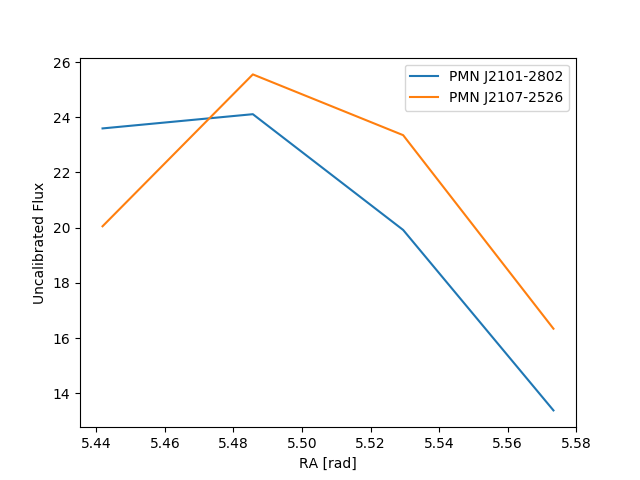
\includegraphics[width=0.47\textwidth]{./2457545_UN_CAL.png}\label{fig:uncal}}
% V_R_3.pdf: 585x441 pixel, 72dpi, 20.64x15.56 cm, bb=0 0 585 441
\subfigure[$B_{kt}^{\nu}$]{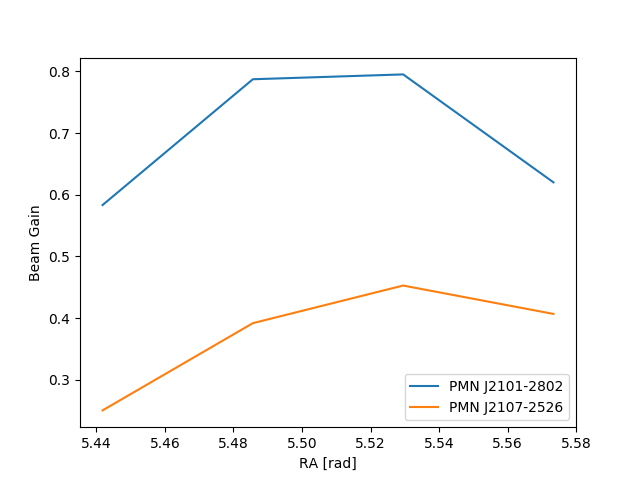
\includegraphics[width=0.47\textwidth]{./2457545_BEAM.png}\label{fig:beam}}
\caption{In this figure we plot the uncalibrated apparent flux of the two absolute flux calibrators (PMN J2101 2802 and PMN J2107 2526) and the primary beam attenuation factor they experience 
at different times (in different snapshots) at 150~MHz. \label{fig:curves}} 
\end{figure}

\begin{figure}
\centering
\subfigure[Galactic center (bandpass and delay calibrator).]{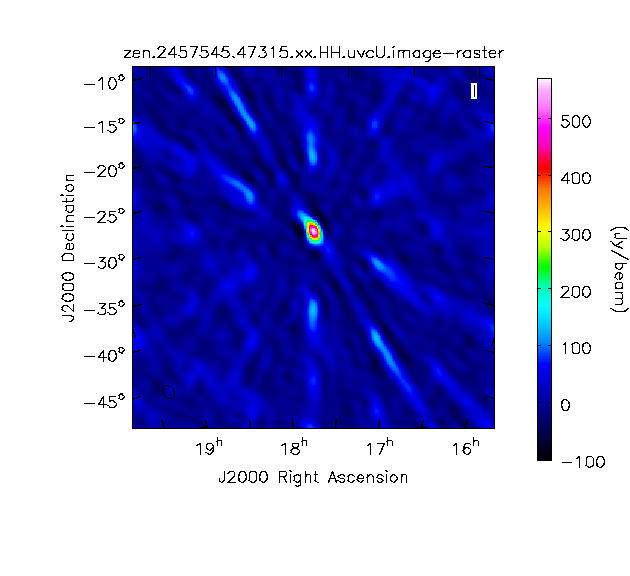
\includegraphics[width=0.47\textwidth]{./GC.png}\label{fig:GC}}
% V_R_3.pdf: 585x441 pixel, 72dpi, 20.64x15.56 cm, bb=0 0 585 441
\subfigure[The two absolute flux calibrators.]{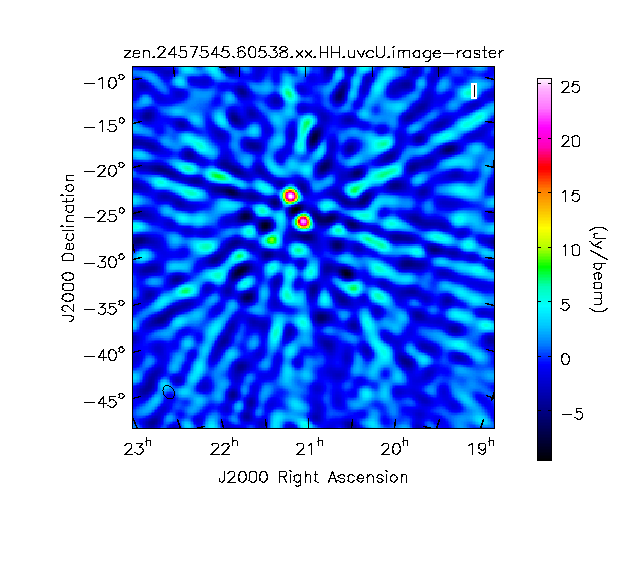
\includegraphics[width=0.47\textwidth]{./2_source.png}\label{fig:two}}
\caption{Absolute flux calibrated images (using Eq.~\eqref{eq:c}) of the Galactic center and the absolute flux calibrators (PMN J2101 2802 and PMN J2107 2526). \label{fig:sources}} 
\end{figure}
%\end{section}
\end{document}
